\documentclass{beamer}
\usepackage[T1]{fontenc}
\usepackage[utf8]{inputenc}
\usepackage{lmodern} 
\usepackage[portuguese]{babel}
\usepackage{graphicx}			%para imagens
\usepackage{epstopdf} 			%resolve problemas eps-pdf
\usepackage{fancyhdr}			% para o cabeçalho bonito
\usepackage{caption}				%para legendas
\usepackage{subcaption}			% e sublegendas
\usepackage{placeins} 			%controlar o lugar dos floats


\usetheme{Warsaw}
\title[Pibic]{Simulação Numérica de Fluidos e Partículas}
\author{Juarez A.S.F.}
\institute{UnB}
\date{24 de Maio, 2013}
\begin{document}
\begin{frame}
\titlepage
\end{frame}
\section{O problema}
\begin{frame}{}
	\frametitle{O Problema}
    \tableofcontents[currentsection,currentsubsection]
 
O que acontece quando passamos fluído por um conjunto de grãos?
\begin{itemize}
 \item<2-> O fluido contorna os grãos individualmente.
 \item<3-> Os grãos são empurrados pelo fluído e se movem.
 \item<4-> Os grãos se movendo colidem entre si.
 \item<5-> E se tivermos muitas partículas?
 \item<6-> O efeito aleatório dessas iterações produz algo interessante.
\end{itemize}
\end{frame}
\begin{frame}{}
	\frametitle{O Problema}
    \tableofcontents[currentsection,currentsubsection]
 
O que acontece quando passamos fluído por um conjunto de grãos?
\begin{itemize}
 \item<2-> O comportamento da mistura dependerá da pressão exercida pelo fluído.
 \item<3-> Em certas condições a mistura passa a se comportar como um outro fluído como um todo
 \item<4-> inclusive respeitando as leis de empuxo de Arquimedes
 \item<5-> Se aumentarmos um pouco mais a velocidade notamos algo estranho
 \item<6-> Surgem ondas de partículas se propagando
\end{itemize}
\end{frame}
\begin{frame}
	\frametitle{O Problema}
    \tableofcontents[currentsection,currentsubsection]
	\begin{block}{Objetivo}
		Nosso objetivo é desenvolver um código que simule a interação flúido-partícula para estudarmos leitos fluidizados
	\end{block}
\end{frame}

\section{A Física}
\begin{frame}{}
	\frametitle{A Física}
    \tableofcontents[currentsection,currentsubsection]
Temos que simular a física de dois processos:
  \begin{itemize}
    \item<2-> Movimento das partículas : 
    \begin{equation}
        \sum \vec{F} = \frac{d}{dt} ( m \cdot \vec{v}(t) )
    \end{equation} 
    \item<3-> Movimento do fluído
    \begin{equation}
		\left\lbrace \begin{tabular}{ll}
				$\frac{\partial u}{\partial t} + u \cdot \nabla u = -\frac{1}{\rho}\nabla p +\nu \nabla ^2 u + F$ \\
				$\nabla \cdot u = 0$
					\end{tabular}		 \right.
    \end{equation} 

  \end{itemize}
\end{frame}

\subsection{A Física das Partículas}
\begin{frame}
	\frametitle{A Física das Partículas}
    \tableofcontents[currentsection,currentsubsection]
	Precisamos determinar as forças externas. São elas:
	\begin{itemize}
		\item<2-> Força peso $\vec{P} = m\vec{g}$
		\item<3-> Força de colisão com outras partículas - como determinar?
			\begin{itemize}
				 \item<4-> resp.: Dinâmica Molecular
			\end{itemize}
	\end{itemize}
\end{frame}
\begin{frame}
	\frametitle{Dinâmica Molecular}
	    \tableofcontents[currentsection,currentsubsection]
	\begin{block}{Dinâmica Molecular}
			Permite pequenas sobreposições(overlaps) das partículas para simular a deformação elástica. Essa superposição é usada junto com outras grandezas físicas para determinar as forças de contado.
	\end{block}
\end{frame}

\begin{frame}
	\frametitle{Dinâmica Molecular}
	   \tableofcontents[currentsection,currentsubsection]
	As principais direções e grandezas são mostrados na figura.
	\begin{figure}
		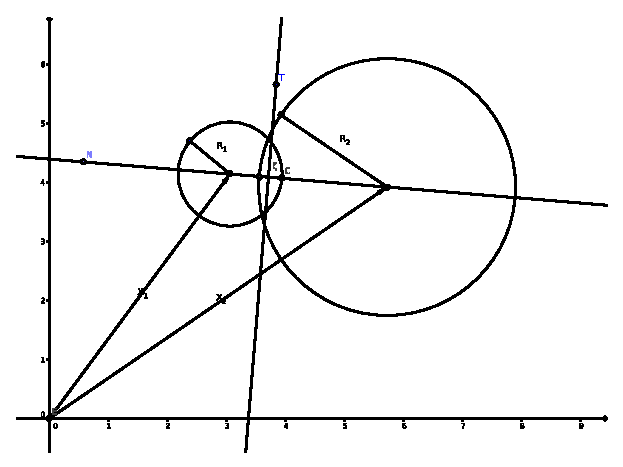
\includegraphics[scale=0.5]{./images/fig_1-1.eps}
		\caption{Quantidades usadas no algoritmo de dinâmica molecular}
		\label{fig:1-1}
	\end{figure}
\end{frame}

\begin{frame}
	\frametitle{Dinâmica Molecular}
	\tableofcontents[currentsection,currentsubsection]
	Definimos:	
	\begin{itemize}
		\item (overlap) $\xi = max(0, R_1 + R_2 - |\vec{x_2} - \vec{x_1} |)$
		\item (direção normal) $\vec{N} = \frac{\vec{x_2} - \vec{x_1} }{|\vec{x_2} - \vec{x_1} |}$
		\item (v de aproximação)$\vec{V} = \vec{v_1} - \vec{v_2}$
		\item (v normal)  $V_n = \dot{\xi} = \vec{V} \cdot \vec{N} $
		\item (v tang.)  $\vec{V}_t = \vec{V} - \dot{\xi}\vec{N} $
	\end{itemize}
\end{frame}

\begin{frame}
	\frametitle{Dinâmica Molecular}
	\tableofcontents[currentsection,currentsubsection]
	\only<2->{ 	Tomando as partículas como perfeitamente lisas em nosso modelo não temos forças na direção tangente e nos preocupamos apenas com a força na direção normal. \\}
	\only<3->{  O modulo da força normal é então dado pela lei de Hook com coeficiente de viscosidade $k_v$ e de restauração elástica$k_r$:}
	\only<4->{	
	\begin{equation}
		\begin{array}{l}
		\vec{F}_n = f_n \vec{N}, \\
		f_n = -(k_v \xi^\alpha \dot{\xi} + k_r \xi^\beta)
		\end{array}
	\end{equation}
	}
\only<5->{
		 onde:
	\begin{itemize}
		\item $k_r$ controla a dureza do material
		\item $k_v$ controla a dissipação durante colisão
	\end{itemize}		
		}
\only<6->
	{
	No caso mais simples tomamos $\beta = 1$ e $\alpha = 0$
	}
\end{frame}

\begin{frame}
	\frametitle{Dinâmica Molecular}
	\tableofcontents[currentsection,currentsubsection]
	\begin{block}{}
		Vemos que com apenas algumas operações vetoriais determinamos as direções das forças de colisão entre partículas. Podemos agora determinar acelerações, velocidades e posições.
	\end{block}
\end{frame}
\begin{frame}
	\frametitle{Dinâmica Molecular}
	\tableofcontents[currentsection,currentsubsection]
	\only<1->
	 {
		O método mais trivial para a integração no tempo é:
		\begin{displaymath}
			\begin{array}{l}
			s^{(n+1)} = s^{(n)} + v^{(n)} \Delta t  	\\
			v^{(n+1)} = v^{(n)} + a^{(n)} \Delta t  	\\
			\end{array}
		\end{displaymath}			 
	 }
\only<2->
	 {
	Existem outros no entanto:
		\begin{displaymath}
			\begin{array}{l}
			s^{(n+1)} = s^{(n-1)} + 2 v^{(n)} \Delta t  	\\
			v^{(n+1)} = v^{(n-1)} + 2 a^{(n)} \Delta t  	\\
			\end{array}
		\end{displaymath}			 
	 }
\only<2->
	{
	Apesar de estranho a princípio pode-se mostrar que o segundo método apresenta convergência mais rápida que o primeiro.
	}
\end{frame}
\begin{frame}
	\frametitle{Dinâmica Molecular - procurando colisões}
	\tableofcontents[currentsection,currentsubsection]
	\only<2->
	{
	Calcular as forças de colisão então é tarefa muito fácil. O problema computacional reside em achar essas colisões!	
	}
	\only<3->
	{
	O método mais óbvio é, para todos os pares de partículas, medir e comparar a distância entre elas com a soma dos raios. Esse método no entanto é O($n^2$) e se torna impraticável para um número grande de partículas	
	}	
	\only<4->
	{
	E se pudéssemos olhar somente as partículas próximas? É claro que as reais candidatas a colisão com uma partícula encontram-se limitadas em um disco centrado no centro dessa partícula e de raio $2 R_{max}$. Mas como fazer isso computacionalmente?
	}
	\only<5->
	{
	Resposta: Tabela Hash
	}		
\end{frame}

\begin{frame}
	\frametitle{Dinâmica Molecular - procurando colisões}
	\tableofcontents[currentsection,currentsubsection]

	\only<2->
	{
	A tabela hash é uma estrutura de dados usada para buscas eficientes. A ideia chave é associar uma chave de comparação de um dado a uma posição na memória. A busca por elementos nessa estrutura é O(1). A função que associa a chave a posição chama-se função de \emph{hashing}.\\
	}		
	\only<3->
	{
	A estrutura é amplamente utilizada em bancos de dados. O google por exemplo utiliza tabelas de dispersão para realizar buscas rápidas.\\
	}
	\only<4->
	{
	Um grande problema ao se implementar uma tabela é achar uma função de dispersão adequada. Idealmente toda chave deve levar a uma posição na memória diferente. Quando chaves diferentes levam em posições iguais ocorre o que chamamos de colisão. Mas isso não é exatamente um problema. \\
	}	
\end{frame}

\begin{frame}
	\only<2->
	{
	Em nosso código a chave de comparação é posição no plano da partícula. A função foi escolhida de forma que pontos próximos do plano sejam levados na mesma memória. Basicamente segmentamos o espaço do $R^2$ em quadrados de lado $R_{max}$\\
	}	
	\only<3->
	{
	A busca com tabelas de dispersão é extremamente eficiente! Mas tudo tem um preço.\\
	}	
	\only<3->
	{
	Em C implementamos a estrutura usando ponteiros, ou seja, trabalhamos com apontadores de endereços de memória. Ponteiros são extremamente eficientes mas quando mal utilizados resultam em falha de segmentação. \\
	}	
	\only<4->
	{
	Basicamente temos uma tebela de listas de ponteiros para partículas. \\
	}	
	\only<5->
	{
	\begin{itemize}
		\item Tabelas são ponteiros para ponteiros
		\item listas são ponteiros enfileirados
		\item o elemento da lista é um ponteiro para partícula
	\end{itemize}	 
	}	
		\only<6->
	{
	Temos um ponteiro para ponteiro para ponteiro para ponteiro de partícula. A busca é O(1), mas a dor de cabeça é O($\infty$)  
	}	
\end{frame}
\section{A física do fluído}
\begin{frame}
	    \begin{equation}
		\left\lbrace \begin{tabular}{ll}
				$\frac{\partial u}{\partial t} + u \cdot \nabla u = -\frac{1}{\rho}\nabla p +\nu \nabla ^2 u + F$ \\
				$\nabla \cdot u = 0$
					\end{tabular}		 \right.
    \end{equation} 
    
    Como resolver?
\end{frame}
\end{document}
